\documentclass[tikz,13pt, crop=true, border=20pt]{standalone}
%\usepackage[english]{babel}
\usepackage[scaled]{helvet}
\renewcommand\familydefault{\sfdefault} 
\usepackage[utf8]{inputenc}
\usepackage{varwidth}
%%%%%%%%%%%%%%%%%%%%%%%%%%%%%%%%%%%%%%%%%%%%%%
%%              MATH
\usepackage{amsmath}
\usepackage{amsthm}
\newtheorem{prop}{Property}
%%%%%%%%%%%%%%%%%%%%%%%%%%%%%%%%%%%%%%%%%%%%%%
%%              CODE AND ALGORITHM
\usepackage{algorithm}
\usepackage{algorithmic}
\usepackage{listings}
        \lstset{frame=tb,
          language=C++,
          aboveskip=3mm,
          belowskip=3mm,
          showstringspaces=false,
          columns=flexible,
          basicstyle={\small\ttfamily},
          numbers=none,
          numberstyle=\tiny\color{gray},
          keywordstyle=\color{blue},
          commentstyle=\color{dkgreen},
          stringstyle=\color{mauve},
          breaklines=true,
          breakatwhitespace=true,
          tabsize=2
        }
%%%%%%%%%%%%%%%%%%%%%%%%%%%%%%%%%%%%%%%%%%%%%%
%%              GRAPHICS
\usepackage{graphicx}
\usepackage{xcolor}
        \definecolor{phase1}{rgb}{0.8,0.2,0.2}
        \definecolor{phase2}{rgb}{0.2,0.8,0.2}
        \definecolor{phase3}{rgb}{0.2,0.2,0.8}
        \definecolor{phase4}{rgb}{0.8,0.2,0.8}
        \definecolor{phase5}{rgb}{1,0.5,0.}
        \definecolor{bananayellow}{rgb}{1.0, 0.88, 0.21}
        %#CC8822 
\usepackage{tikz}
\usetikzlibrary{arrows, calc}
        % usage: \tikzpic{<x percent>}{<y percent>}{<image size>}{<image name>}
        \newcommand*{\tikzpic}[4]{%
        \begin{tikzpicture}[remember picture,overlay]
        \node at (current page.south west) [xshift=#1\paperwidth,yshift=#2\paperheight] {\includegraphics[width=#3\linewidth]{#4}};
        \end{tikzpicture}%
        }
        \usetikzlibrary{shapes,arrows,positioning}
        %% TIKZ DEFINITIONS
        \tikzstyle{data} = [rectangle, draw, fill=none,%
                  text centered, minimum height=4em, ultra thick,
                  execute at begin node={\begin{varwidth}{25em}\centering{\small\textless\textless memory\textgreater\textgreater\\}},%
                  execute at end node={\end{varwidth}}]
        \tikzstyle{op} = [rectangle, rounded corners = 20pt, draw, fill=none,%
                  text centered, minimum height=4em, ultra thick,%
                  execute at begin node={\begin{varwidth}{25em}\centering{\small\textless\textless compute\textgreater\textgreater\\}},%
                  execute at end node={\end{varwidth}}]
        \tikzstyle{line} = [draw, -latex']

\graphicspath{{../images/}}
\usepackage{epsfig}
\usepackage{epstopdf}
\usepackage{placeins}
%%%%%%%%%%%%%%%%%%%%%%%%%%%%%%%%%%%%%%%%%%%%%%%%%%
%%	     IF ELSE THEN
\usepackage{ifthen}
%\ifthenelse{\equal{#3}{sq} \OR #3 > 0}
%           {... valid ...}
%           {... invalid ...}
%%%%%%%%%%%%%%%%%%%%%%%%%%%%%%%%%%%%%%%%%%%%%%%%%%
%%           TITLEPAGE DEFINITION
\title{}
\date{}
%%%%%%%%%%%%%%%%%%%%%%%%%%%%%%%%%%%%%%%%%%%%%%%%%%%%%%%%%%%%%%%%
\newcount\xpos
\newcount\ypos

\begin{document}

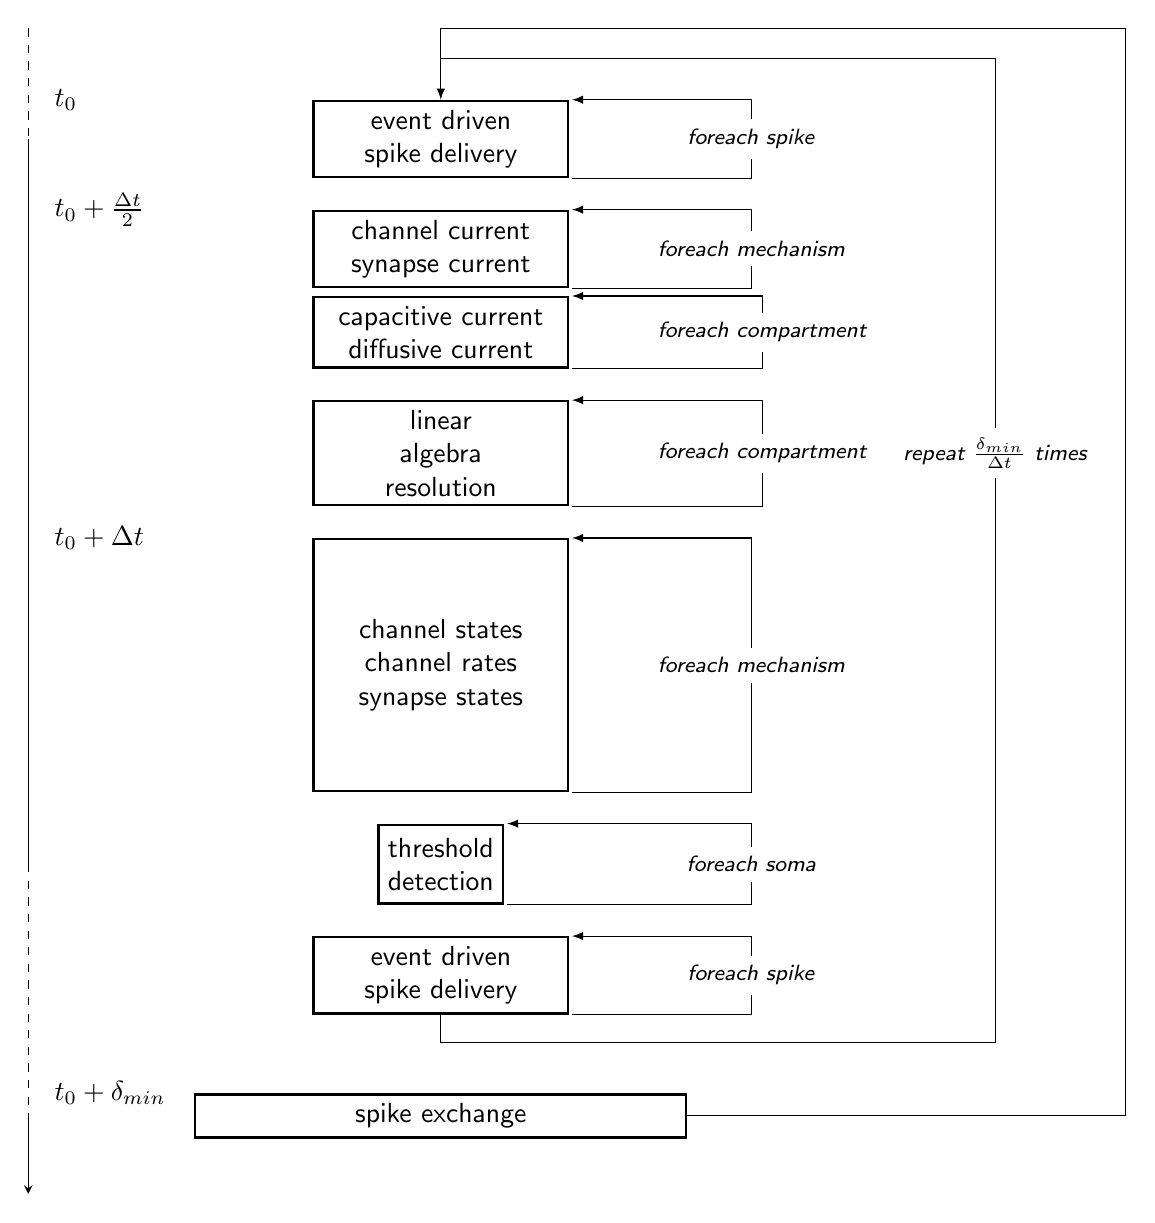
\begin{tikzpicture}

%----------------------------------------------------------------------------------------------------------------
%\node[draw=none, align = center] at (-1,2.5)  {Task-based representation of the minimum delay loop\\in a hybrid clock-event driven implementation of a compartmental model.};
%----------------------------------------------------------------------------------------------------------------

\node[rectangle, thick,draw, text width = 3cm, align = center] (sd) at (-2.95,0)  {event driven\\spike delivery};
\node[rectangle, thick,draw, text width = 3cm, align = center, anchor = north, below = 0.4cm of sd] (ch)  {channel current \\ synapse current};
\node[rectangle, thick, draw, text width = 3cm, align = center, anchor = north, below = 0.1cm of ch, minimum height = 0.6cm] (cap) {capacitive current\\diffusive current};
\node[rectangle, thick, draw, text width = 3cm, align = center, anchor = north, below = 0.4cm of cap, minimum height = 0.6cm] (tri)  {linear\\algebra\\resolution};
\node[rectangle, thick, draw, text width=3cm, align = center, minimum height = 3.2cm, anchor = north, below = 0.4cm of tri] (nonvint) {channel states\\ channel rates\\synapse states};
\node[rectangle, thick, draw, text width=1.35cm, anchor=north, align = center, minimum height = 1cm, anchor = north, below = 0.4cm of nonvint] (thr)  {threshold\\detection};
\node[rectangle, thick,draw, text width = 3cm, align = center, anchor = north, below = 0.4cm of thr] (sd2) {event driven\\spike delivery};

%----------------------------------------------------------------------------------------------------------------

\node[draw = none, anchor = west, right = of ch] (chfor) {\footnotesize \emph{foreach mechanism}};
\draw ([xshift=1pt]ch.south east) -| (chfor.south);
\draw[->, >=latex] (chfor.north) |- ([xshift=1pt]ch.north east);
\node[draw = none, anchor = west, right = of cap] (capfor) {\footnotesize \emph{foreach compartment}};
\draw ([xshift=1pt]cap.south east) -| (capfor.south);
\draw[->, >=latex] (capfor.north) |- ([xshift=1pt]cap.north east);
\node[draw = none, anchor = west, right = of tri] (trifor) {\footnotesize \emph{foreach compartment}};
\draw ([xshift=1pt]tri.south east) -| (trifor.south);
\draw[->, >=latex] (trifor.north) |- ([xshift=1pt]tri.north east);
%\node[draw = none, anchor = west, right = of bks] (bksfor) {\footnotesize \emph{repeat foreach compartment}};
%\draw (bks.south east) -| (bksfor.south);
%\draw[->, >=latex] (bksfor.north) |- (bks.north east);
\node[draw = none, anchor = west, right = of nonvint] (nonvintfor) {\footnotesize \emph{foreach mechanism}};
\draw ([xshift=1pt]nonvint.south east) -| (nonvintfor.south);
\draw[->, >=latex] (nonvintfor.north) |- ([xshift=1pt]nonvint.north east);
\path let \p1 = (nonvintfor.south), \p2 = (thr) in node[draw = none] (thrfor) at (\x1, \y2) {\footnotesize \emph{foreach soma}};
\draw ([xshift=1pt]thr.south east) -| (thrfor.south);
\draw[->, >=latex] (thrfor.north) |- ([xshift=1pt]thr.north east);
\path let \p1 = (nonvintfor.south), \p2 = (sd) in node[draw = none] (sdfor) at (\x1, \y2) {\footnotesize \emph{foreach spike}};
\draw ([xshift=1pt]sd.south east) -| (sdfor.south);
\draw[->, >=latex] (sdfor.north) |- ([xshift=1pt]sd.north east);
\path let \p1 = (nonvintfor.south), \p2 = (sd2) in node[draw = none] (sd2for) at (\x1, \y2) {\footnotesize \emph{foreach spike}};
\draw ([xshift=1pt]sd2.south east) -| (sd2for.south);
\draw[->, >=latex] (sd2for.north) |- ([xshift=1pt]sd2.north east);
\node[draw = none, anchor = west, right = 0.2cm of trifor] (dtrepeat) {\footnotesize \emph{repeat $\frac{\delta_{min}}{\Delta t}$ times}};
\draw let \p1 = (dtrepeat.south), \p2 = (sd2.south) in (sd2.south) |- (\x1, \y2 - 10) -- (dtrepeat.south);
%\draw[->, >=latex] (dtrepeat.north) |- (sd.east);
\draw let \p1 = (sd.north) in (dtrepeat.north) |- (\x1, \y1 + 15);

%----------------------------------------------------------------------------------------------------------------
%%\node[rectangle, thick,rotate=90, draw, text width = 3cm, align = center] (sd2) at (-2.95,-10)  {event driven\\spike delivery};

%%\node[rectangle, thick,rotate=90, draw, text width = 3cm, align = center] (ch2) at (-1.65,-10)  {channel current \\ syanpse current};
%\node[rectangle, thick,rotate=90, draw, text width = 3cm, align = center] at (-1.4,-10) {synapse current};
%%\node[rectangle, thick,rotate=90, draw, text width = 3cm, align = center] (cap2) at (-0.8,-10) {capacitance};

%%\node[rectangle, thick,rotate=90, draw, text width = 3cm, align = center] (tri2) at (0,-10)  {triangularization};
%%\node[rectangle, thick,rotate=90, draw, text width = 3cm, align = center] (bks2) at (0.6,-10) {back substitution};

%%\node[rectangle, thick, draw, text width=1.35cm, anchor=north, align = center, minimum height = 1cm, rotate=90] (thr2) at (4.275,-10)  {threshold\\detection};

%%\node[rectangle, thick, draw, text width=3cm, align = center, minimum height = 3.2cm, rotate=90] (nonvint2) at (2.6,-10)  {channel states\\ channel rates\\synapse states};

%\draw [dashed, thick] (5.95,-2) -- (5.95,2.3);
%%\draw [thick] (5.95,-10) -- (7.5,-10);

%%\node [diamond, thick, draw, text width = 1.2cm, align = center] (delay2) at (7.5,-7.5) {exceed\\min delay};

%%\draw [thick,->] (7.5,-10) -- (delay2.south);

%%\draw [thick,->] (delay2.west) -| (sd2.east);
%%\draw [thick,->] (delay2.north) |- (comm.north);

%%\node [draw = none, anchor=north east] at (delay2.west) {{\small \emph{no}}};
%%\node [draw = none, anchor=south west] at (delay2.north) {{\small \emph{yes}}};

%----------------------------------------------------------------------------------------------------------------

\node [rectangle, draw, thick, text width = 6cm, align = center, anchor = north, below = 1cm of sd2] (comm) {spike exchange};% \\ \textbf{barrier}};
\draw[->, >=latex] let \p1 = (sd.east), \p2=(dtrepeat.east) in (comm.east) -| (\x2 + 10, \y1 + 40 ) -| (sd.north);

%----------------------------------------------------------------------------------------------------------------
\draw let \p1 = (sd.west), \p2 = (thr.west),\p3 = (comm.west) in (\x3 - 60, \y1) -- (\x3 - 60, \y2 ) ;
\draw[dashed] let \p1 = (comm), \p2 = (thr.west), \p3 = (comm.west) in (\x3 - 60, \y2) -- (\x3 - 60, \y1 ) ;
\draw[dashed] let \p1 = (sd.west), \p2 = (thr.south west), \p3 = (comm.west) in (\x3 - 60, \y1+40) -- (\x3 - 60, \y1 ) ;
\draw[->, >=stealth] let \p1 = (comm), \p2 = (thr.south west), \p3 = (comm.south west) in (\x3 - 60, \y1) -- (\x3 - 60, \y3 - 20) ;

\path let \p1 = (comm.west), \p2 = (sd.north west) in node[draw = none, anchor = east, text width=1.5cm] at (\x1-0.15cm, \y2) {$t_0$};
\path let \p1 = (comm.west), \p2 = (ch.north west) in node[draw = none, anchor = east, text width=1.5cm] at (\x1-0.15cm, \y2) {$t_0 + \frac{\Delta t}{2}$};
%\path let \p1 = (comm.west), \p2 = (cap.west) in node[draw = none, anchor = east, text width=1.5cm] at (\x1-0.15cm, \y2) {$t_0 + \frac{\Delta t}{2}$};
%\path let \p1 = (comm.west), \p2 = (tri.west) in node[draw = none, anchor = east, text width=1.5cm] at (\x1-0.15cm, \y2) {$t_0 + \frac{\Delta t}{2}$};
%\path let \p1 = (comm.west), \p2 = (bks.west) in node[draw = none, anchor = east, text width=1.5cm] at (\x1-0.15cm, \y2) {$t_0 + \frac{\Delta t}{2}$};
\path let \p1 = (comm.west), \p2 = (nonvint.north west) in node[draw = none, anchor = east, text width=1.5cm] at (\x1-0.15cm, \y2) {$t_0 + \Delta t$};
%\path let \p1 = (comm.west), \p2 = (thr.west) in node[draw = none, anchor = east, text width=1.5cm] at (\x1-0.15cm, \y2) {$t_0 + \Delta t$};
\path let \p1 = (comm.west), \p2 = (comm.north west) in node[draw = none, anchor = east, text width=1.5cm] at (\x1-0.15cm, \y2) {$t_0 + \delta_{min}$};


%----------------------------------------------------------------------------------------------------------------
%%\draw[thick, dashed]
%%let
%%    \p1 = (sd.north east),
%%    \p2 = (delay.south)
%%  in
%%    (\x1 - 10.0, \y1 + 20.0) rectangle (\x2 + 50, \y2 - 15)
%%    node[draw = none, anchor = west] at (\x1, \y2) {\small \emph{thread \#1}};
%%
%%
%%\draw[thick, dashed]
%%let
%%    \p1 = (sd2.north west),
%%    \p2 = (delay2.north) 
%%  in
%%    (\x1 - 10.0, \y1 - 20.0) rectangle (\x2 + 50, \y2 + 15)
%%    node[draw = none, anchor = west] at (\x1, \y2) {\small \emph{thread \#2}};

%----------------------------------------------------------------------------------------------------------------
%\node [draw = none, anchor = south] at (-2.95, 1.7) {\footnotesize$t_n$};

%\node [draw = none, anchor = south] at (-1.4, 1.7) {\footnotesize$t_{n+1/2}$};
%\node [draw = none, anchor = south] at (0.3, 1.7) {\footnotesize$t_{n+1/2}$};

%\node [draw = none, anchor = south] at (2.6, 1.7) {\footnotesize$t_{n+1}$};
%\node [draw = none, anchor = south] at (5, 1.7) {\footnotesize$t_{n+1}$};

%----------------------------------------------------------------------------------------------------------------

%%\draw[thick, ->] let \p1 = (comm.west) in (comm.west) -- (\x1, \y1 - 100) -| (sd2.west);
%%\draw[thick, ->] let \p1 = (comm.east) in (comm.east) -- (\x1, \y1 + 100) -| (sd.east);

%----------------------------------------------------------------------------------------------------------------

%%\draw[->] let \p1 = (ch2.west) in plot [smooth, tension=2] coordinates {(ch2.south west) (\x1, \y1 - 10)  (ch2.north west)};
%%\draw[->] let \p1 = (cap2.west) in plot [smooth, tension=2] coordinates {(cap2.south west) (\x1, \y1 - 10)  (cap2.north west)};
%%\draw[->] let \p1 = (tri2.west) in plot [smooth, tension=2] coordinates {(tri2.south west) (\x1, \y1 - 10)  (tri2.north west)};
%%\draw[->] let \p1 = (bks2.west) in plot [smooth, tension=2] coordinates {(bks2.south west) (\x1, \y1 - 10)  (bks2.north west)};
%%\draw[->] let \p1 = (nonvint2.south) in plot [smooth, tension=2] coordinates {(nonvint2.south east) (\x1, \y1 - 10)  (nonvint2.south west)};
%\draw[->] let \p1 = (thr2.south) in plot [smooth, tension=2] coordinates {(thr2.south east) (\x1, \y1 - 10)  (thr2.south west)};

%%\draw[->] let \p1 = (ch.west) in plot [smooth, tension=2] coordinates {(ch.south west) (\x1, \y1 - 10)  (ch.north west)};% node[draw = none, anchor=north] at (\x1, \y1 - 8) {\footnotesize \emph{mech}};
%%\draw[->] let \p1 = (cap.west) in plot [smooth, tension=2] coordinates {(cap.south west) (\x1, \y1 - 10)  (cap.north west)};% node[draw = none, anchor=north] at (\x1, \y1 - 8) {\footnotesize \emph{node}};;
%%\draw[->] let \p1 = (tri.west) in plot [smooth, tension=2] coordinates {(tri.south west) (\x1, \y1 - 10)  (tri.north west)};
%%\draw[->] let \p1 = (bks.west) in plot [smooth, tension=2] coordinates {(bks.south west) (\x1, \y1 - 10)  (bks.north west)};
%%\draw[->] let \p1 = (nonvint.south) in plot [smooth, tension=2] coordinates {(nonvint.south east) (\x1, \y1 - 10)  (nonvint.south west)};
%\draw[->] let \p1 = (thr.south) in plot [smooth, tension=2] coordinates {(thr.south east) (\x1, \y1 - 10)  (thr.south west)};

%%\node[draw = none, anchor=north] at (ch2.west) {\footnotesize \emph{m}};
%%\node[draw = none, anchor=north] at (cap2.west) {\footnotesize \emph{c}};
%%\node[draw = none, anchor=north] at (tri2.west) {\footnotesize \emph{c}};
%%\node[draw = none, anchor=north] at (bks2.west) {\footnotesize \emph{c}};
%%\node[draw = none, anchor=north] at (nonvint2.south) {\footnotesize \emph{m}};

%%\node[draw = none, anchor=north] at (ch.west) {\footnotesize \emph{m}};
%%\node[draw = none, anchor=north] at (cap.west) {\footnotesize \emph{c}};
%%\node[draw = none, anchor=north] at (tri.west) {\footnotesize \emph{c}};
%%\node[draw = none, anchor=north] at (bks.west) {\footnotesize \emph{c}};
%%\node[draw = none, anchor=north] at (nonvint.south) {\footnotesize \emph{m}};

\end{tikzpicture}

\end{document}













